\section{Spectral GNNs}

\begin{frame}{Spectral GNNs}
    \destaq{Introduction to Spectral GNNs}
    \begin{itemize}
        \item Spectral Graph Neural Networks derived from GSP principles.
        \item \textbf{Key Concept}: Graph Laplacian $\mathcal{L} = D - A$ (degree matrix $D$ and adjacency matrix $A$) captures graph structure, enabling spectral operations analogous to Fourier transforms.
        \item Objective: Represent node features as signals on a graph.
        \item Spectral Methods:
        \begin{itemize}
            \item \textbf{Eigenvalue-based}: Filters created in Fourier domain.
            \item \textbf{Eigenvector-based}: Decomposition of signals via spectral basis \cite{bo2023surveyspectralgraphneural}.
        \end{itemize}
    \end{itemize}
\end{frame}

\begin{frame}{Spectral CNN (SCNN)}
    \destaq{First Spectral GNN - Spectral CNN (SCNN)}
    \begin{itemize}
        \item \textbf{Concept}: Transforms CNN concepts from images to graphs.
        \item \textbf{Mathematics}:
        \begin{itemize}
            \item Graph Fourier Transform: $\hat{f} = U^T f$
            \item Convolution: $g_{\theta} \star f = U g_{\theta} U^T f$, where $U$ and $\Lambda$ are derived from $\mathcal{L} = U \Lambda U^T$.
            \item \textbf{Challenges}:
            \begin{itemize}
                \item High computational cost $\mathcal{O}(n^3)$.
                \item Non-localized eigenvectors can overshadow local details \cite{bruna2013spectral}.
            \end{itemize}
        \end{itemize}
    \end{itemize}
\end{frame}

\begin{frame}{Graph Laplacian Spectra}
    \begin{figure}
      \begin{columns}
        \column{.3\linewidth}
        \caption{Eigenvectors as signals denotes nodal regions of eigenvalues of the graph Laplacian.}
        \label{fig:graph_spectra}
        \column{.65\linewidth}
        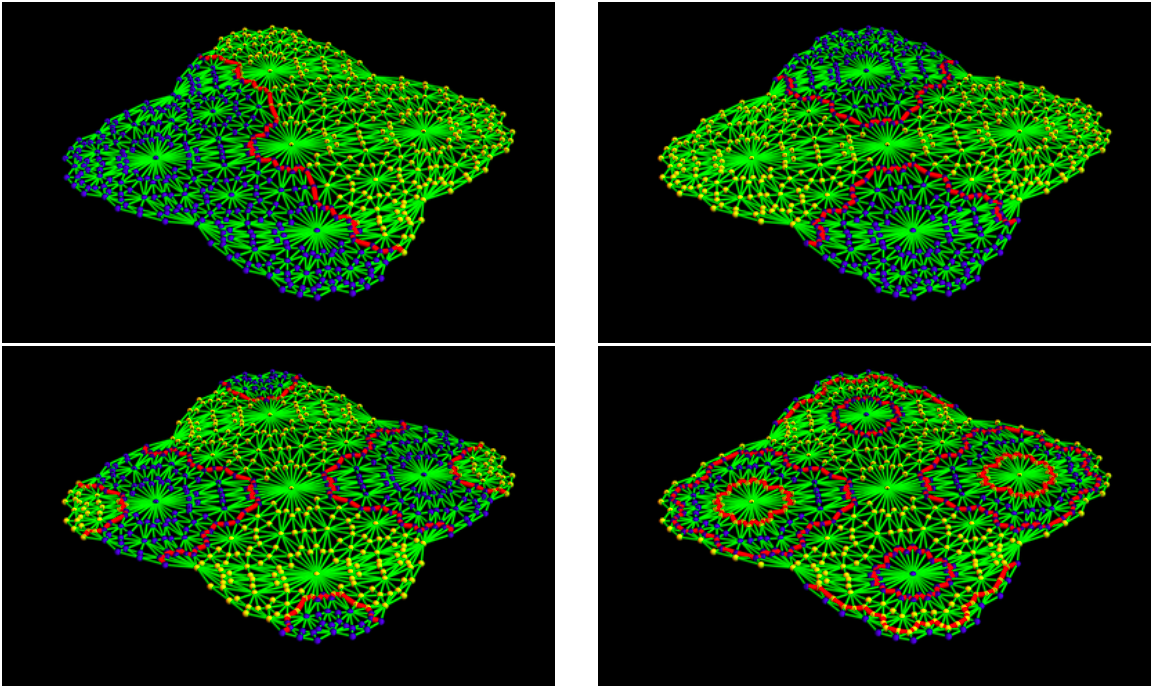
\includegraphics[width=\textwidth]{img/graph_spectra.png}
      \end{columns}
    \end{figure}

\end{frame}


\begin{frame}{ChebNet}
    \destaq{ChebNet - Addressing SCNN Limitations}
    \begin{itemize}
        \item \textbf{Introduction of Chebyshev Polynomials}:
        \begin{itemize}
            \item Approximates spectral filters for reduced computational demands using Chebyshev polynomials.
            \item Defines filters as: $ g_{\theta}(\mathcal{L} ) f = \sum_{k=0}^{K-1} \theta_k T_k(\widetilde{\mathcal{L}}) f $.
            \item Scaled Laplacian: $\widetilde{\mathcal{L}} = 2 \frac{\mathcal{L}}{\lambda_\text{max}} - I_n$.
        \end{itemize}
        \item \textbf{Advantages}:
        \begin{itemize}
            \item \textbf{Scalability}: Only first eigenpair needed ($\mathcal{O}(n^2)$ via power method).
            \item \textbf{Localized Filtering}: $K$-localized for $K^{th}$-order polynomial filters, representing paths up to length $K$ \cite{defferrard2016convolutional}.
        \end{itemize}
    \end{itemize}
\end{frame}

\begin{frame}{Graph Convolutional Networks (GCNs)}
    \destaq{Graph Convolutional Networks (GCNs) - A Simplified Approach}
    \begin{itemize}
        \item \textbf{GCN Concept}:
        \begin{itemize}
            \item Rooted in Chebyshev expansion truncation ($K=1$), focusing on first-order neighbors.
            \item Propagation Rule: $g_{\theta} \star f \approx \theta (I_n + \widetilde{A}) f$ with $\widetilde{A} = D^{-\frac{1}{2}} A D^{-\frac{1}{2}}$.
        \end{itemize}
        \item \textbf{Benefits}:
        \begin{itemize}
            \item Simplifies computation while remaining effective.
            \item Often categorized as a spatial method due to neighborhood aggregation \cite{kipf2016semi}, \cite{wu2019simplifying}.
        \end{itemize}
    \end{itemize}
\end{frame}

\begin{frame}{GCN diagram}
    \begin{figure}[h]
    \centering
    \begin{columns}

    \column{.25\linewidth}

    \caption{Graph Convolution updating node embedding $\vec{h_b}$}

    \label{fig:visualgo}

    \column{.75\linewidth}
    \resizebox{0.975\columnwidth}{0.455\linewidth}{%

\begin{tikzpicture}[scale=1.8, auto,swap]
    \foreach \pos/\name in {{(0,2)/a}, {(2,1)/b}, {(4,1)/c},
                            {(0,0)/d}, {(3,0)/e}, {(2,-1)/f}, {(4,-1)/g}}
        \node[vertex] (\name) at \pos {};
        
    \foreach \source/ \dest /\weight in {b/a/7, c/b/8,d/a/5,d/b/9,
                                         e/b/7, e/c/5,e/d/15,
                                         f/d/6,f/e/8,
                                         g/e/9,g/f/11}
        \path[edge] (\source) -- (\dest);
         
    \foreach \vertex / \fr in {b/4}
        \path node[selected vertex] at (\vertex) {$\vec{h}_b$};
    \foreach \vertex / \fr in {a/4, c/4, d/4, e/5}
        \path node[select vertex] at (\vertex) {$\vec{h}_{\vertex}$};
    \begin{pgfonlayer}{background}
        \foreach \source / \dest in {b/c,d/b,a/b,b/e}
            \path[selected edge] (\source.center) -- (\dest.center);
    \end{pgfonlayer}
    
    \foreach \pos/\name in {{(6,2)/a1}, {(8,1)/b1}, {(10,1)/c1},
                            {(6,0)/d1}, {(9,0)/e1}, {(8,-1)/f1}, {(10,-1)/g1}}
        \node[vertex] (\name) at \pos {};
    \foreach \source/ \dest /\weight in {b1/a1/7, c1/b1/8,d1/a1/5,d1/b1/9,
                                         e1/b1/7, e1/c1/5,e1/d1/15,
                                         f1/d1/6,f1/e1/8,
                                         g1/e1/9,g1/f1/11}
        \path[edge] (\source) -- (\dest);
    \foreach \vertex / \fr in {b1/4}
        \path node[selectx vertex] at (\vertex) {$\vec{h}'_b$};
        
    \draw[-stealth, densely dotted, ultra thick, mygreen] (b) edge[bend left=20] (b1);
\end{tikzpicture}


}
\end{columns}
\end{figure}
\end{frame}

\begin{frame}{Limitations of Spectral Methods}
    \destaq{Limitations of Spectral Methods}
    \begin{itemize}
        \item Restriction: Spectral GNNs typically work only on undirected graphs as they rely on symmetric spectral decomposition.

        \item Scalability: GCNs apart, spectral methods tend to be computationally expensive for large graphs.

        \item The nature of the adjacency matrix enforces `node-centric' approaches that may not be suitable for all tasks.

    \end{itemize}
\end{frame}